\section{ $ $ $ $ Shared task on word sense induction}

\subsection{}

\begin{frame}{A shared task on WSI}
  
  \begin{itemize}
  \item An \textbf{\alert{ACL SIGSLAV}} sponsored shared task on \textbf{word sense induction} (WSI) for the Russian language.
 \end{itemize} 
  
  \begin{itemize}
    \item \textbf{More details}: \url{https://russe.nlpub.org/2018/wsi}
     
  \end{itemize}
  
  \begin{center}
  	
\includegraphics[width=0.2\textwidth]{figures/acl}
  \end{center}
  
   \begin{center}
  	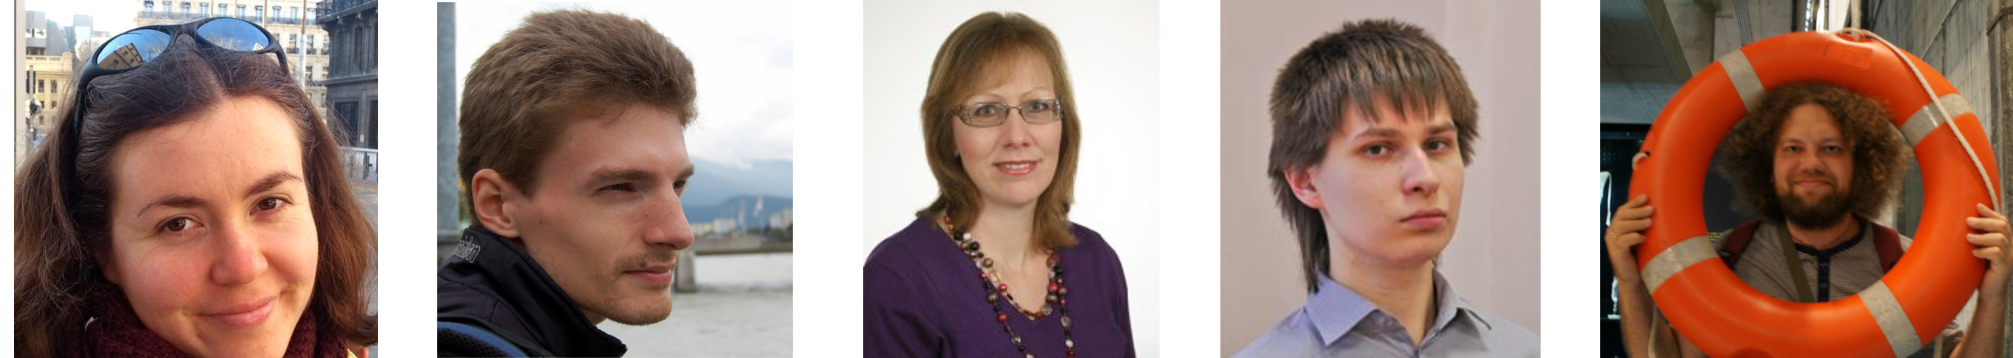
\includegraphics[width=0.99\textwidth]{figures/russe-team}
  \end{center}
\end{frame}



\begin{frame}{A lexical sample WSI task}
  
  \begin{itemize}
  	\item \textbf{Target word}, e.g. ``bank''.
  	
  	\pause 
  	
  	\item \textbf{Contexts} where the word occurs, e.g.: 
  	\begin{itemize}
  	\item ``river \textbf{bank} is a slope beside a body of water''
  	\item ``\textbf{bank} is a financial institution that accepts deposits''
  	\item ``Oh, the \textbf{bank} was robbed. They took about a million dollars.''
  	\item ``\textbf{bank} of Elbe is a good and popular hangout spot complete with good food and fun''
  	\end{itemize}
  	
  	\pause 
  	
  	\item You need to \textbf{{group} the contexts by senses}:
  	\begin{itemize}
  	\item \textcolor{Cerulean}{``river \textbf{bank} is a slope beside a body of water''}
  	\item \textcolor{Cerulean}{``\textbf{bank} of Elbe is a good and popular hangout spot complete with good food and fun''}
  	\item \alert{``\textbf{bank} is a financial institution that accepts deposits''}
  	\item \alert{``Oh, the \textbf{bank} was robbed. They took about a million dollars.''}
  	\end{itemize}
  	 
  \end{itemize}
  
\end{frame}


\begin{frame}{Dataset based on Wikipedia}

{\centering
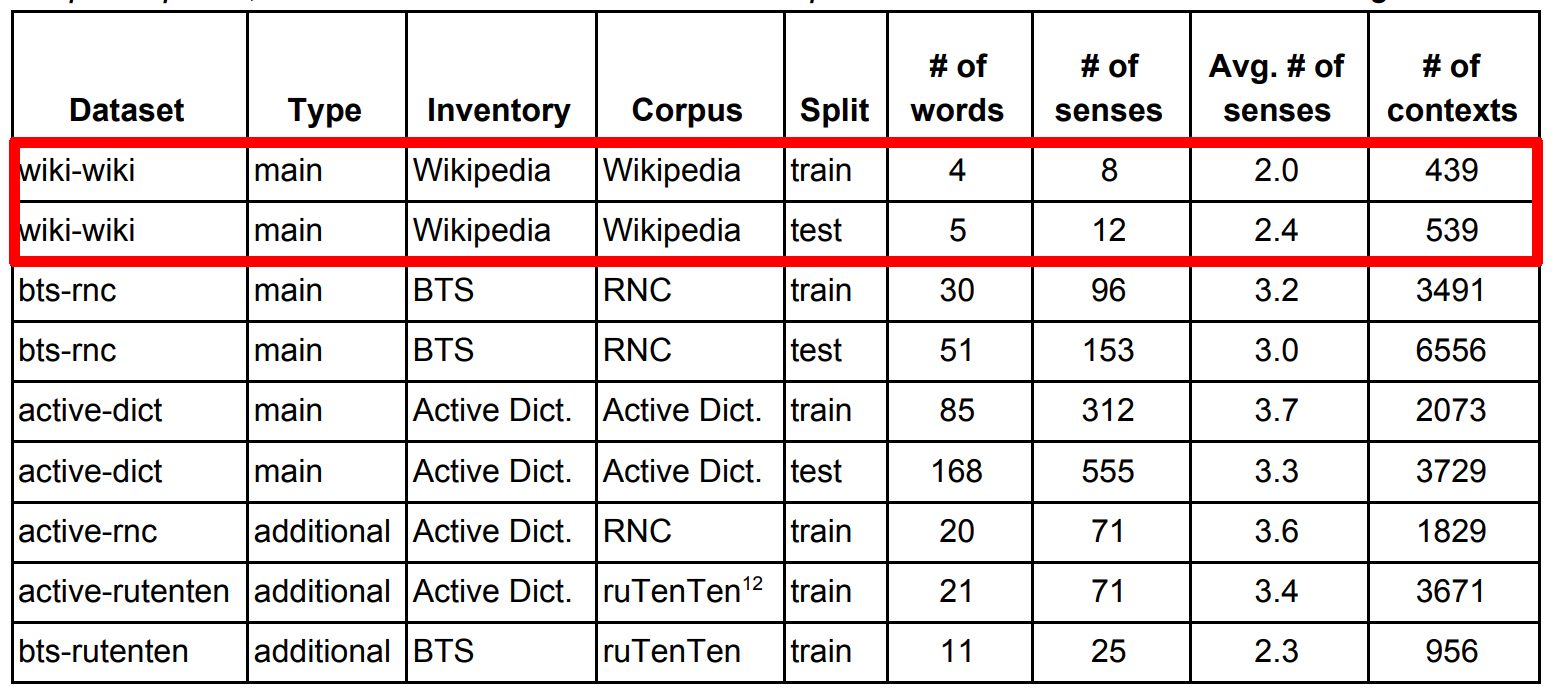
\includegraphics[width=1.0\textwidth]{figures/datasets1}
}	
\end{frame}


\begin{frame}{Dataset based on RNC}

{\centering
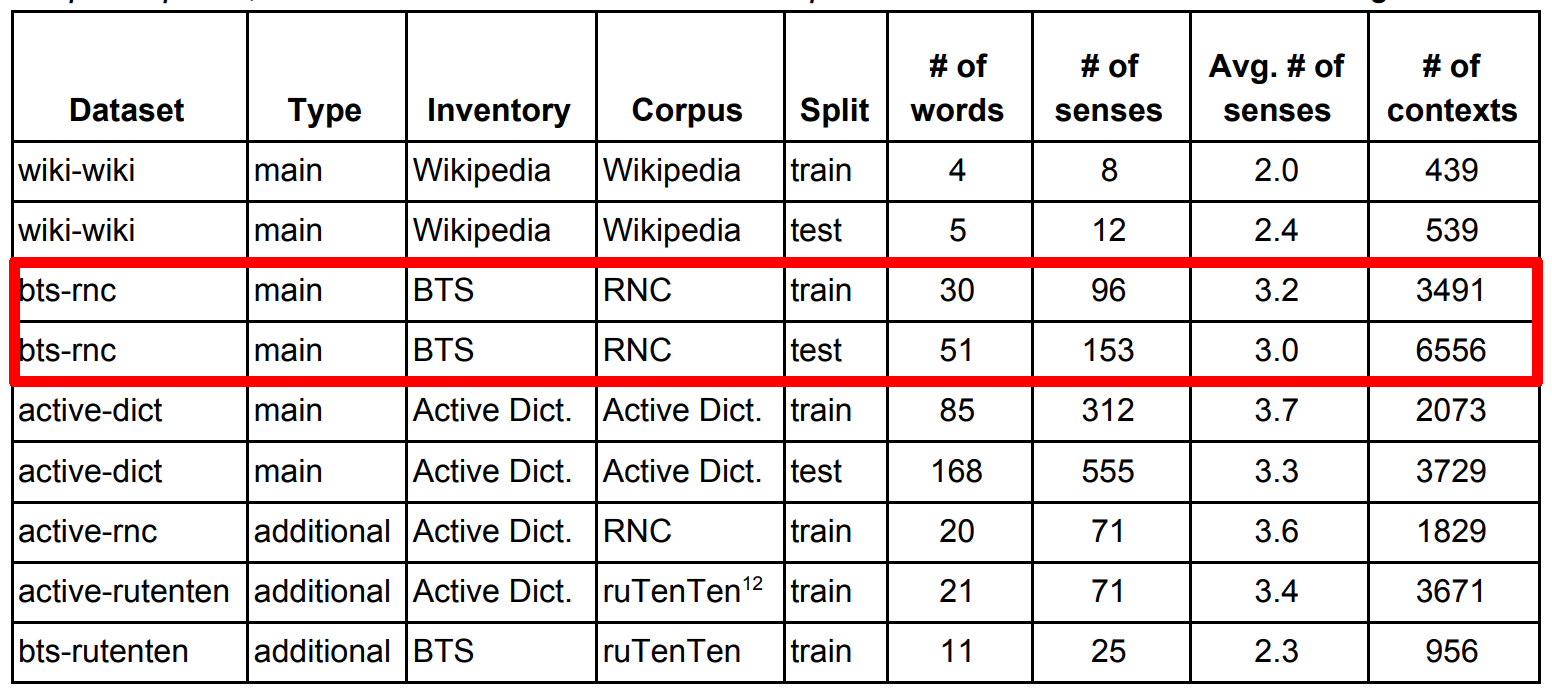
\includegraphics[width=1.0\textwidth]{figures/datasets2}
}	
\end{frame}


\begin{frame}{Dataset based on dictionary glosses}

{\centering
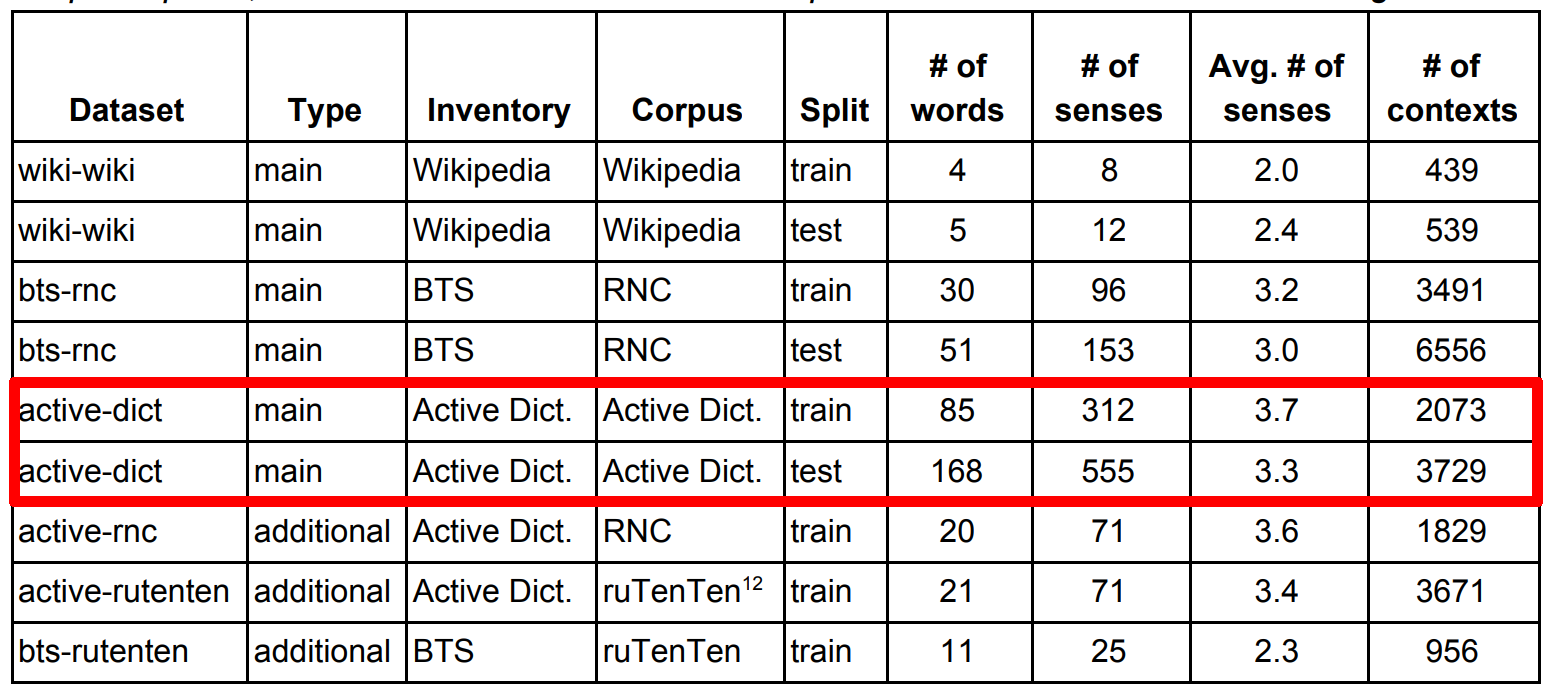
\includegraphics[width=1.0\textwidth]{figures/datasets3}
}	
\end{frame}



\begin{frame}{A sample from the \textit{wiki-wiki} dataset }

{\centering
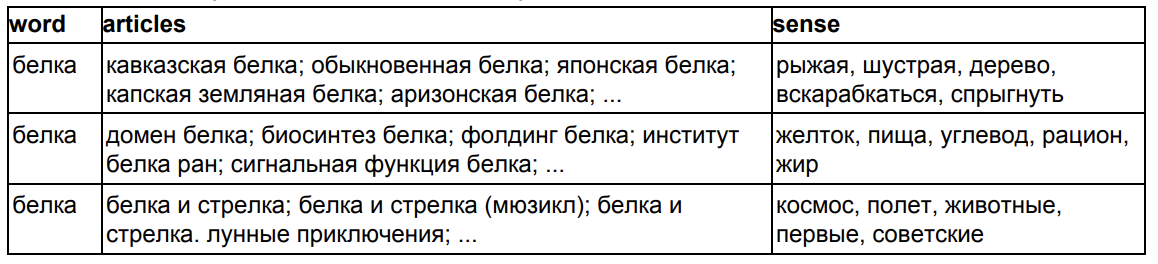
\includegraphics[width=1.0\textwidth]{figures/belka}
}	
\end{frame}



\begin{frame}{A sample from the \textit{wiki-wiki} dataset }

{\centering
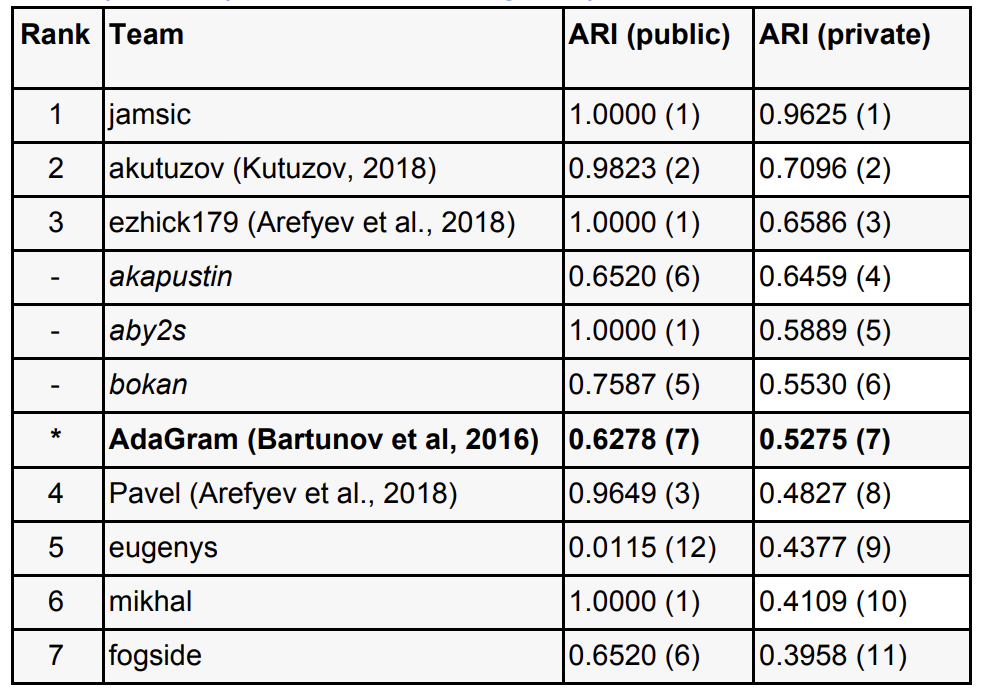
\includegraphics[width=.8\textwidth]{figures/wiki-wiki}
}	
\end{frame}



\begin{frame}{A sample from the \textit{wiki-wiki} dataset }

{\centering
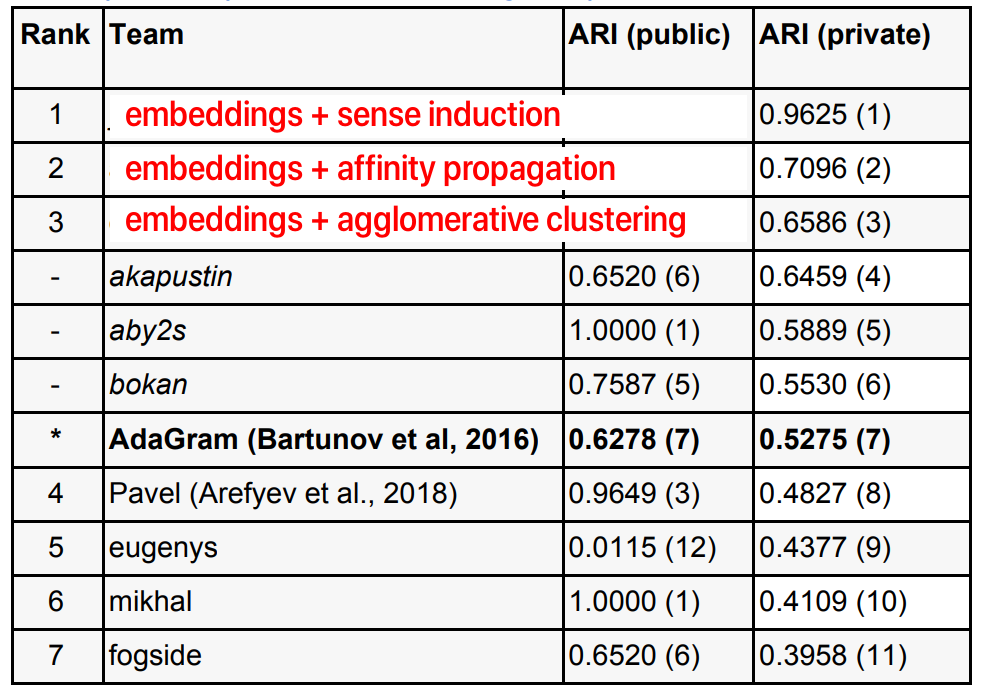
\includegraphics[width=.8\textwidth]{figures/wiki-wiki-top}
}	
\end{frame}



\begin{frame}{A sample from the \textit{bts-rnc} dataset }

{\centering
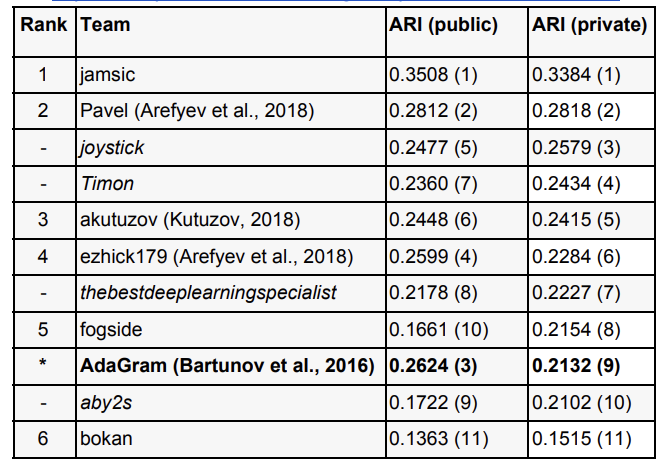
\includegraphics[width=.8\textwidth]{figures/bts}
}	
\end{frame}



\begin{frame}{A sample from the \textit{active-dict} dataset }

{\centering
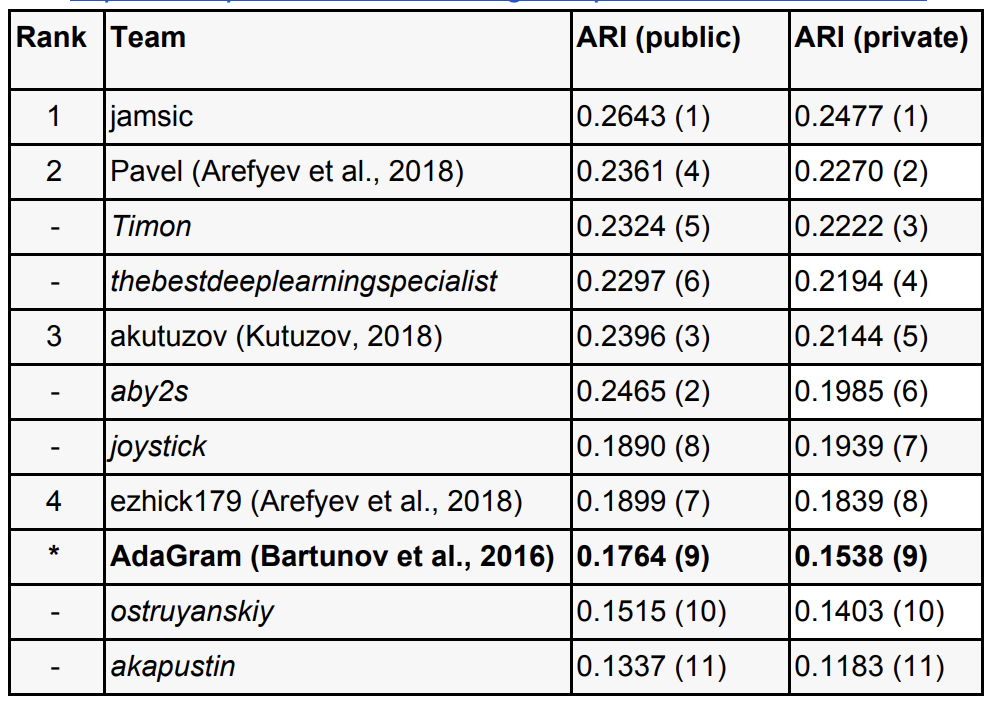
\includegraphics[width=.8\textwidth]{figures/active}
}	
\end{frame}



\begin{frame}{ \textit{jamsic}: sense induction }

\begin{enumerate}
	\item \textbf{Get the neighbors} of a target word, e.g. \textbf{``bank''}:
	\begin{enumerate}
	\item \alert{lender}
	\item \textcolor{Cerulean}{river}
	\item \alert{citybank}
	\item \textcolor{Cerulean}{slope}
	\item ...
	\end{enumerate}
	
	\item Get \textbf{similar to ``bank''} and \textbf{dissimilar to \alert{``lender''}}:
	
	\begin{enumerate}
	\item \textcolor{Cerulean}{river}
	\item \textcolor{Cerulean}{slope}
	\item \textcolor{Cerulean}{land}
	\item ...
	\end{enumerate}
	 
\item \textbf{Compute distances} to \alert{\textbf{``lender''}} and \textcolor{Cerulean}{\textbf{``river''}}.
\end{enumerate}

\end{frame}


